\label{chapter-scenario-template}
\textbf{Created by:} Perawit Charoenwut \\
\textbf{Modified by:}

\subsection*{Scenario Objective}
This scenario illustrates how to represent a complete company structure with manufacturing and business divisions using the IOF core ontology. It focuses on:
\begin{itemize}
    \item Showing how business and manufacturing units coexist within one company
    \item Distinguishing between business and manufacturing activities
    \item Capturing different organizational roles and functions
\end{itemize}

\subsection*{General Pattern Description}
A company can contain both business organizations and manufacturers as part of its structure.
An Organization can simultaneously be:
\begin{enumerate}
    \item A BusinessOrganization that has a BusinessFunction, which is realized through a SellingBusinessProcess that sells the MaterialProduct
    \item A Manufacturer that has a ManufacturerRole, which is realized through a ProductProductionProcess and  has the MaterialProduct as its output.
\end{enumerate}

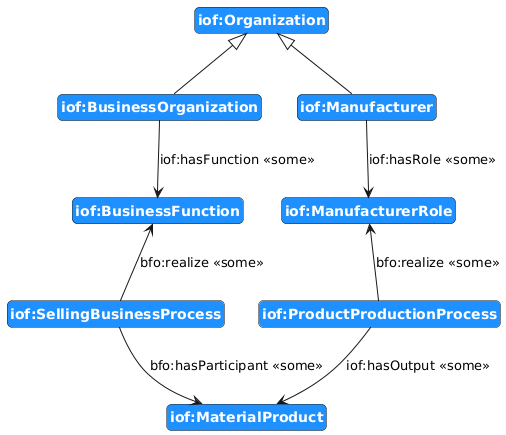
\includegraphics[scale=0.42]{scenarios/different-type-organizations/image/different-type-organizations-schema}

\subsection*{Use Case: }

This use case demonstrates how a company like GE operates as both a manufacturer and a business organization using the same material products.

\subsubsection*{Use-Case Pattern Description}
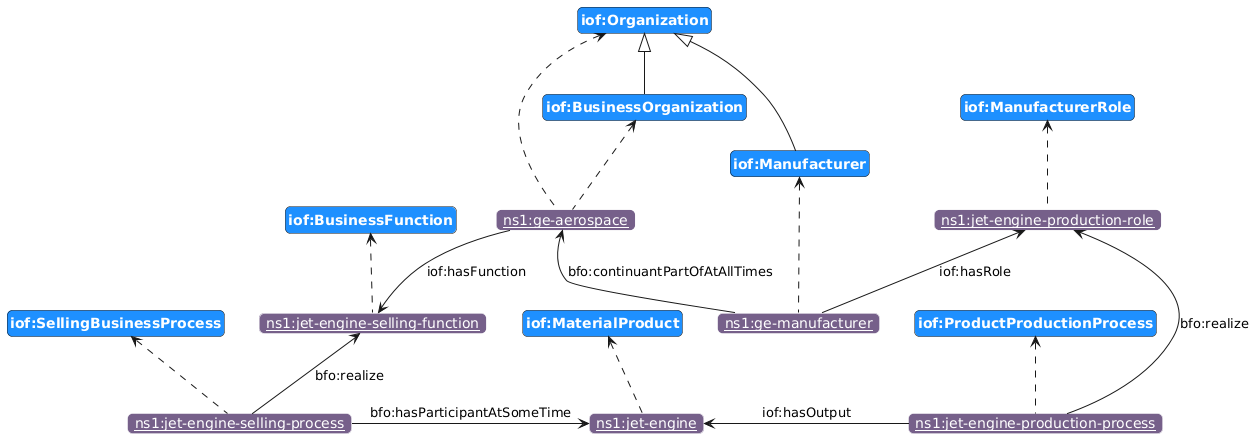
\includegraphics[scale=0.4]{scenarios/different-type-organizations/image/different-type-organizations}

GE Aerospace (\texttt{iof:Organization}) operates as both a manufacturer and a business organization (\texttt{iof: BusinessOrganization}) with respect to jet engines(\texttt{iof:MaterialProduct}). As a manufacturer (\texttt{iof:Manufacturer}), GE Aerospace bears \texttt{iof:ManufacturerRole} which is \texttt{bfo:realize} through \texttt{iof:ProductProductionProcess}, producing jet engines as \texttt{iof:MaterialProduct}. The same organization is a business organization by having \texttt{iof:BusinessFunction} which is \texttt{bfo:realize} through \texttt{iof:SellingBusinessProcess}, where the same jet engines \texttt{are bfo:hasParticipantAtSomeTime} in the selling process.

\subsubsection*{Use-Case Example Data}


\begin{table}[h]
% \caption{}
\label{tab:organization-structure}
% \resizebox{\columnwidth}{!}{%
\begin{tabular}{|l|l|}
\hline
Entity & Function/Role \\ \hline
GE Aerospace & Manufactures and sells product \\
Jet engine & Product \\
Manufacturing & Manufactures product \\
Sales & Sells product \\
\hline
\end{tabular}%
% }
\end{table}


\subsubsection*{Data Mapping}


\subsubsection*{Data Validation}
